%\documentclass[francais,a4paper]{scrartcl}
%

\textbf{Consignes}

\input{../../../exos/consignes/consignes_TP4}


\activite{Bataille navale}

\question{} Dans le jeu de la bataille navale, on représente chaque case par un couple d'entiers entre 0 et~9.

Un navire a ses extrémités sur les cases \pyv{a} et \pyv{b}. Un joueur tire sur la case \pyv{x}. 

\'Ecrire une fonction \pyv{touche(a,b,x)} qui renvoie un booléen indiquant si le navire est touché ou non.


\activite{Simulation d'un prêt immobilier}

Un banquier vous  propose un prêt de $400\,000$ euros  sur $40$ ans «à
$3\%$ par  an» ---  ce qui, dans  le langage commercial  des banquiers,
veut  dire $0,25\%$  par mois  ---  avec des  mensualités de  $1431,93$
euros.  Autrement  dit,  vous   contractez  une  dette  de  $400\,000$
euros. Chaque mois, cette dette  augmente de $0,25\%$ puis est diminuée
du  montant  de  votre  mensualité.  À  la  fin  des  $40  \times  12$
mensualités, il  ne vous  reste plus qu'à  vous acquitter  d'une toute
petite dette, que vous rembourserez aussitôt.


\question{} Écrire  une fonction  \pyv{reste_a_payer(p, t,  m, d)}
renvoyant  le montant  de cette  somme à  rembourser  immédiatement
après le paiement de la dernière
mensualité, où  $p$ est le  montant total du  prêt en euros (dans l'exemple, $400\,000$), $t$ son  taux mensuel (dans l'exemple, 
$0,25 \times 10^{-2}$), $m$ le montant d'une mensualité en euros (dans l'exemple, $1431,93$) et $d$ la
durée en années (dans l'exemple, $40$).

\emph{Indice : dans le cas donné dans cet énoncé, vous devez trouver un montant
restant d'un peu moins de $7,12$ euros.}


\question{} Écrire une fonction \pyv{somme_totale_payee(p, t, m,
  d)} renvoyant la somme totale (mensualités plus le dernier
paiement) que vous aurez payé au banquier.


\question{}Écrire une fonction \pyv{cout_total(p, t, m, d)} renvoyant
  le coût total  du crédit, c'est-à-dire le total de  ce que vous avez
  payé moins le montant du prêt.
  
Un banquier vous propose de vous prêter $p$ euros, à un taux de $12t\%$ par an ---  ce qui, dans  le langage commercial  des banquiers,
veut  dire $t\%$  par mois  --- avec des  mensualités de  $m$ euros. Autrement  dit,  vous   contractez  une  dette  de  $p$
euros. Chaque mois, cette dette  augmente de $t\%$ puis est diminuée du  montant  de  votre  mensualité. Lorsque votre dette, augmentée du taux, est inférieure à la mensualité, il suffit de régler le solde en une fois.

\question{} \'Ecrire une fonction \pyv{duree_mensualite(p,t,m)} renvoyant le nombre de mensualités nécessaires au remboursement total du prêt.

\question{} Attention : que se passe-t-il si la mensualité est trop petite ? 

\emph{Indice : dans le cas où le prêt est $\texttt{p}=4\times10^5$, le taux est $\texttt{t}=0,25\times10^{-2}$ et la mensualité est $\texttt{m}=1431,93$, on trouvera une durée de remboursement de $480$ mois.}

\question{} \'Ecrire une fonction \pyv{tracer_amortissement(p,t,m)} permettant de tracer pour les tous mois jusqu'à ce que le prêt soit remboursé le capital restant du ainsi que la somme cumulé des intérêts versé à la banque.



\activite{Suites}

 On pose $u_{0} = 1$ et pour tout $n\in \N$,
\begin{align*}
  u_{n+1} &= \frac{1}{2}\p{u_{n}+\frac{n+1}{u_{n}}}\\
\text{et } v_{n} &= \sum_{k=0}^{n} \frac{1}{u_{k}^{5}}
\end{align*}

\question{} Écrire une fonction \pyv{f(n)} renvoyant la valeur de
  $v_{n}$.

On peut montrer que $\p{v_{n}}_{n\in \N}$ converge.

\textbf{Attention}: on fera attention à ce que le calcul de \pyv{f}
de demande  pas trop de (re)calculs inutiles. Pour fixer les idées,
vous  pouvez considérer  que  \pyv{f(10**6)} doit être calculé  en
(largement) moins d'une minute.

\question{} Vérifier que vous pouvez calculer $v_{n}$ pour de grandes valeurs de $n$.




\activite{ (Facultative) Sommes}

\question{} Écrire une fonction \pyv{somme1(n)} et une fonction \pyv{somme2(n)} prenant en argument
un entier naturel \pyv{n} et renvoyant respectivement
\begin{gather}
  \sum_{1\leq i,j\leq n} \frac{1}{i+j^{2}}~, \\
  \sum_{1\leq i<j\leq n} \frac{1}{i+j^{2}}~.
\end{gather}

Au besoin, on introduira des fonctions auxiliaires.

%\title{Informatique tronc commun TP 01}
%\date{6 septembre 2018}
%\begin{document}
%\maketitle{}

\begin{multicols}{2}
Cette séance commencera par une présentation du fonctionnement d'un ordinateur (Partie~\ref{sec.ordi}). 
La seconde partie de la séance sera consacrée au TP en lui-même (Partie~\ref{sec.demontage}) : vous 
démonterez les anciens ordinateurs du lycée pour repérer et étudier leurs composants. 

\begin{enumerate}
\item  \textbf{Lisez attentivement  tout l'énoncé
    avant de commencer.}
\item Après la séance, vous devez rédiger un compte-rendu de TP et
l'envoyer au format électronique à votre enseignant.
\item Le seul format accepté pour l'envoi d'un texte de compte-rendu est le
format PDF. Votre fichier s'appellera impérativement \texttt{tp01\_berne\_durif.pdf}, où \og \texttt{berne}\fg\ et \og \texttt{durif}\fg\ sont à remplacer par les noms des membres du binôme. 
\item Ce TP est à faire en binôme, vous ne rendrez donc qu'un
  compte-rendu pour deux.
\item Pensez à vous munir d'un appareil photo (un smartphone est suffisant).
\item Avant d'envoyer le compte rendu, merci de vérifier que les photos incluses dedans sont d'un poids raisonnable.
\end{enumerate}


\section*{Généralités sur le fonctionnement d'un ordinateur.}\label{sec.ordi}

\subsection*{Qu'est-ce qu'un ordinateur?}

C'est une machine
\begin{itemize}
\item Servant à traiter de l'information
\item Programmable
\item Universelle
\end{itemize}

\subsubsection*{Exemples/contre-exemples}

\begin{enumerate}
\item Automobile
\item Thermostat d'ambiance (mécanique)
\item Thermostat d'ambiance (électronique)
\item Téléphone portable (smartphone)
\item PC de bureau
\item Lecteur MP3
\item Box de votre FAI
\end{enumerate}

\subsubsection*{Universalité}
\begin{center}
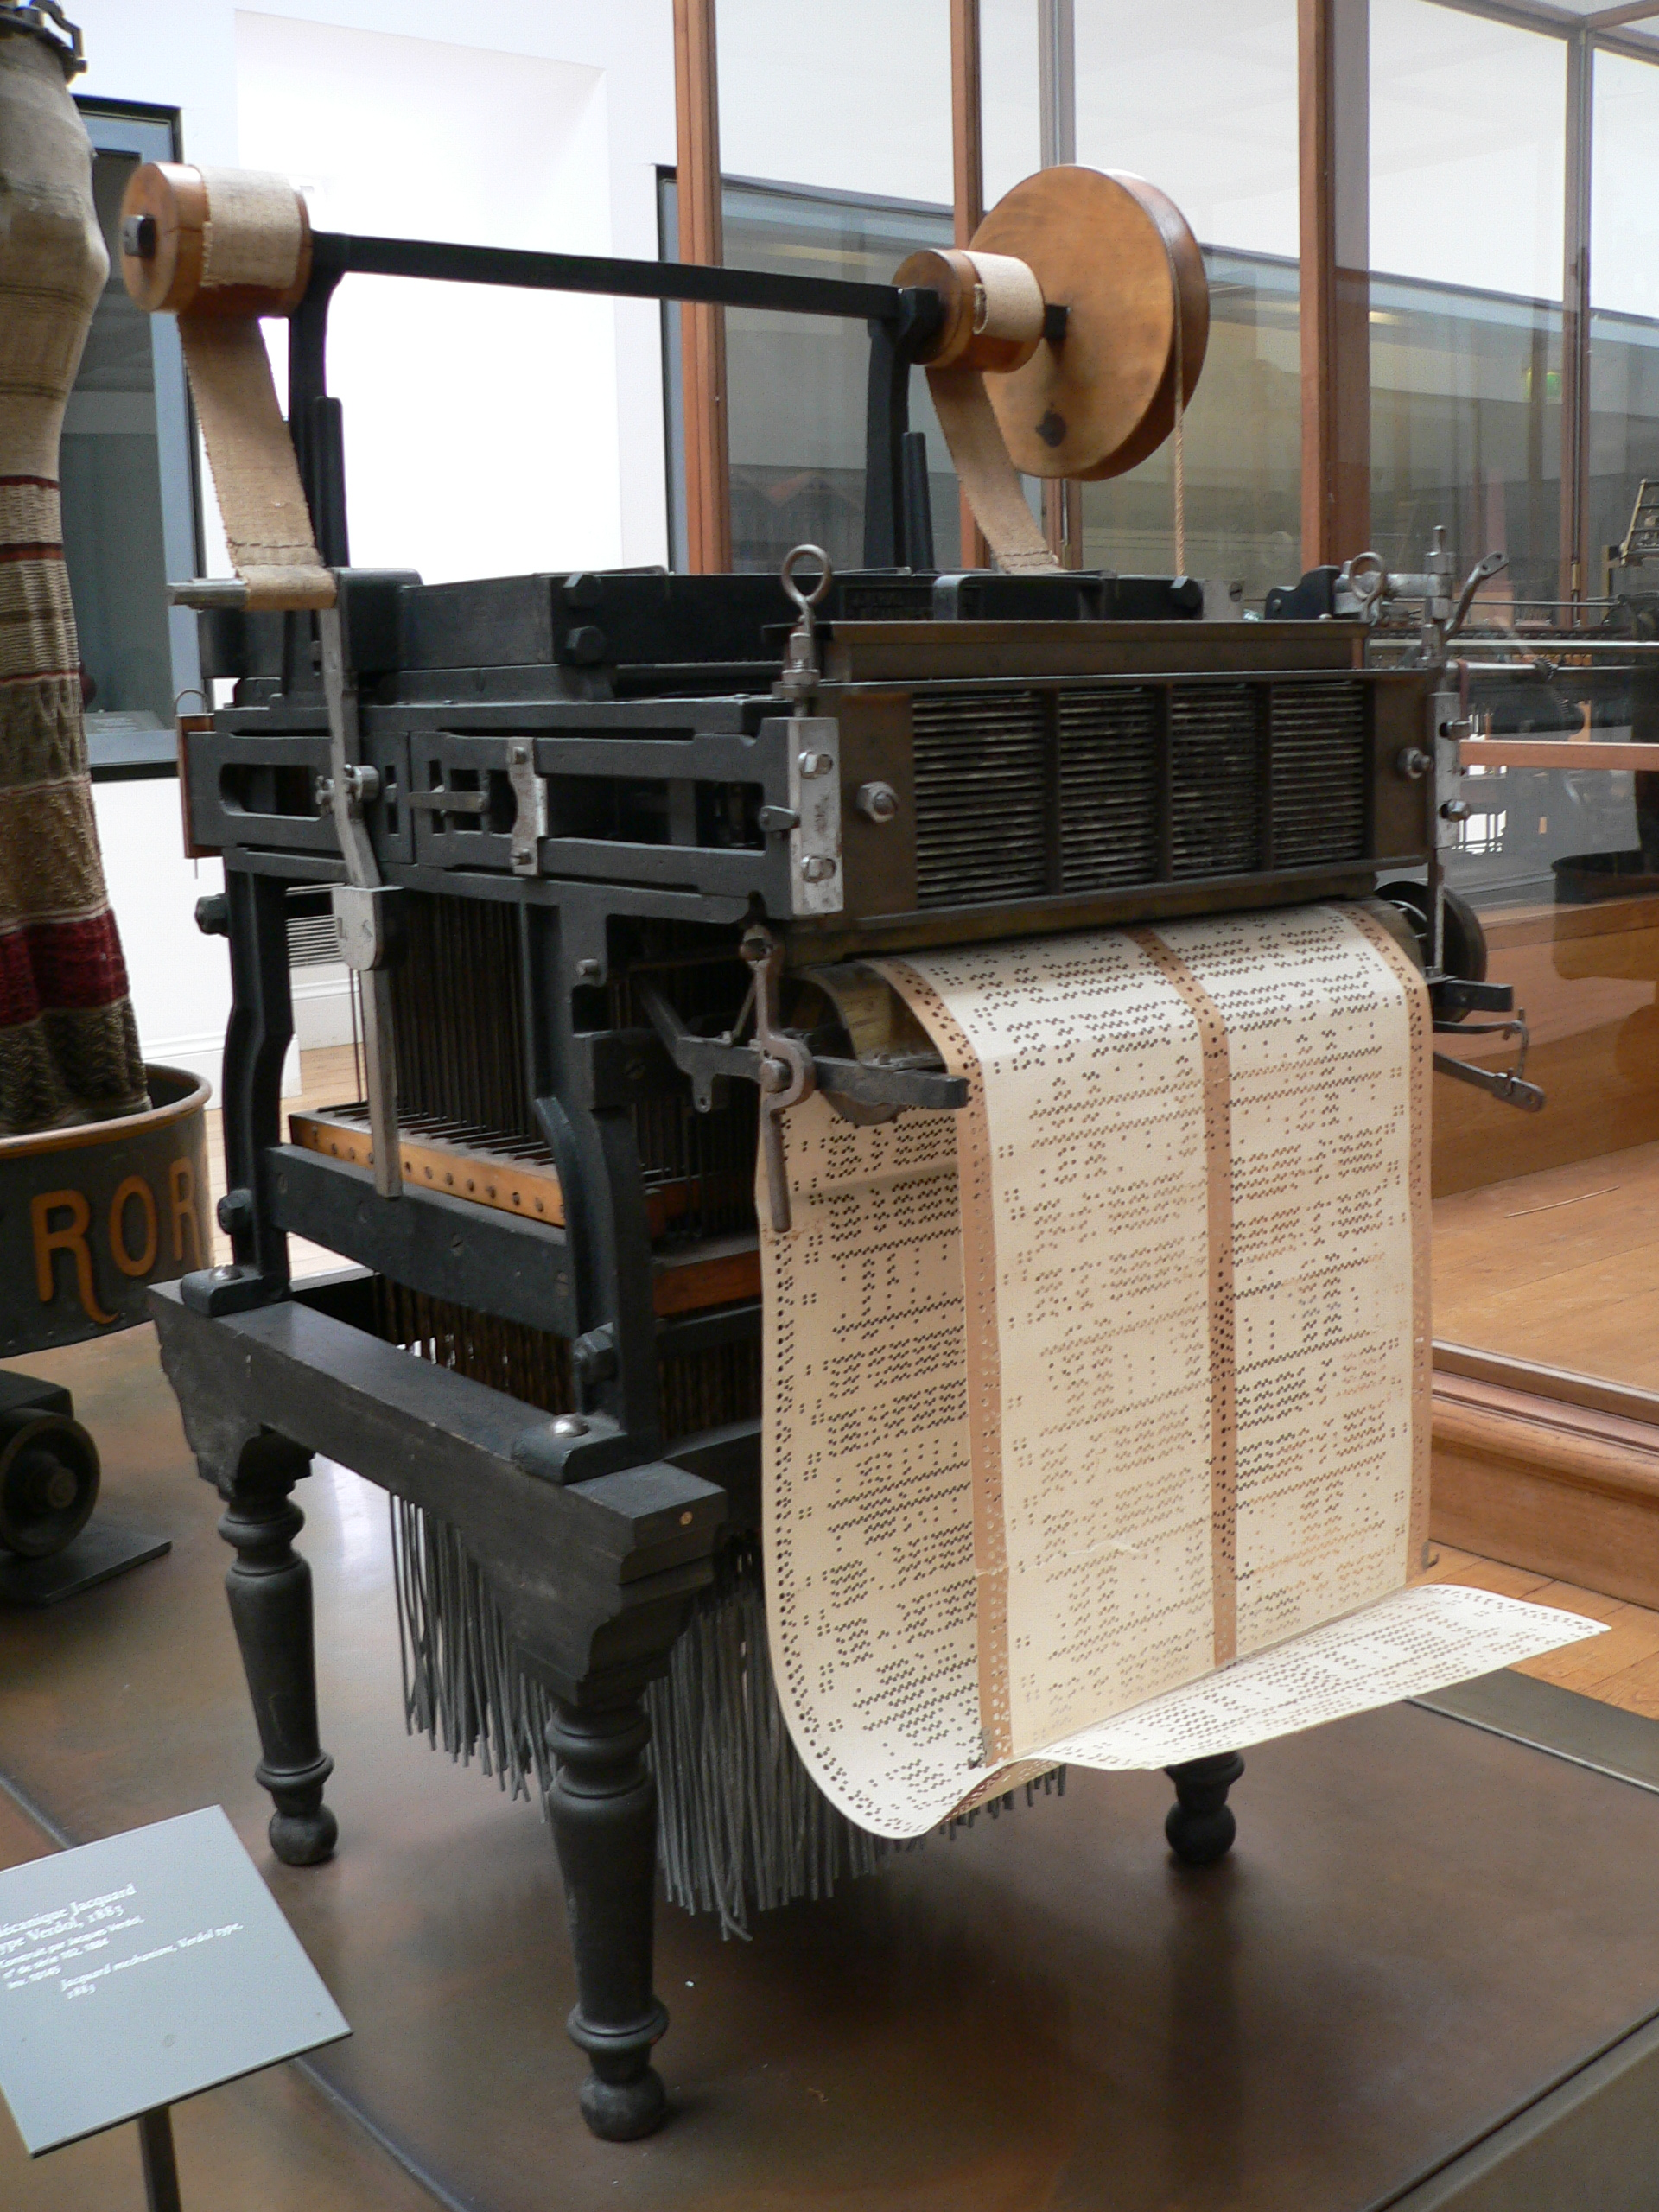
\includegraphics[width=3cm]{metier-jacquard.jpg}
\end{center}
%\begin{minipage}[b]{0.5\linewidth}
  Ce métier Jacquard :
  \begin{itemize}
  \item traite de l'information ;
  \item est programmable ;
  \item mais n'est pas une machine \emph{universelle} !
  \end{itemize}
%\end{minipage}

\begin{defi}
Définition informelle : universelle $=$ «capable de calculer toute fonction exprimable par un
algorithme».
%\end{quote}

Définition mathématique : universelle $=$ «capable de calculer toute fonction calculable par
  une machine de Turing».
Une machine de Turing est un dispositif abstrait, que nous ne détaillerons pas ici. 
\end{defi}

\subsection*{Architecture de von Neumann}

\begin{itemize}
\item Version concrète d'une machine de Turing universelle.
\item Modèle architectural de tous les ordinateurs depuis 70 ans.
\end{itemize}

\begin{figure}[!h]
\centering
\begin{tikzpicture}
\tikzset{cadre/.style={minimum width=3.75cm,minimum height=3cm,rectangle,rounded
corners=7.5pt,draw,fill=blue!7.5,font=\bfseries}}
\tikzset{pcadre/.style={minimum width=3cm,minimum
height=.6cm,rectangle,draw,font=\bfseries}}
\tikzset{mcadre/.style={minimum
width=.75cm,minimum height=.6cm,rectangle,draw,font=\bfseries}}
%\tikzset{fleche/.style={>=triangle 90,line width=.6cm,color=gray!10}}
\tikzset{fleche/.style={fill=gray!15, single arrow, draw=none,minimum
    width=1.5cm, minimum height=3.225cm,single arrow head extend=0.0525cm}}
\tikzset{pfleche/.style={>=stealth,thick}}
\node[cadre] (U) at(-3.75,0){};
\node[cadre] (M) at (3.75,0){\begin{minipage}{3cm}
\begin{center}
Mémoire à accès direct\\
(RAM et ROM)
\end{center}\end{minipage}};
\node[cadre, minimum height=1.75cm] (P) at (0,-2.7){Périphériques
  (réseau, disques durs, écran, clavier\ldots{})};
%\draw[fleche,->] (0,0)--(P);
%\draw[fleche,<->](U)--(M);
%\node [fleche, double arrow, minimum height=5cm]{Bus};
\node[fleche] at (0,0){};
\node[rotate=-90,fleche,minimum height=1.6cm] at (0,-0.75){};
\node[rotate=+180,fleche] at (0,0){};
\draw[font=\bfseries] (0,0) node{Bus};
\node[pcadre](Uc) at (-3.75,0.9){Unité de contrôle};
\node[mcadre](R0) at (-4.875 ,.3){$R_0$};
\node[mcadre](R1) at (- 4.125,.3){$R_1$};
\node[mcadre](Rd) at (- 3.375,.3){$\dots$};
\node[mcadre](Rn) at (- 2.625,.3){$R_n$};
\node[pcadre](Ual) at (-3.75,-0.9) {UAL};
\draw[pfleche,->](R1)--+(0,-0.9);
\draw[pfleche,<-](Rd)--+(0,-0.9);
\end{tikzpicture}
\caption{Architecture de von Neumann}
\end{figure}


Mémoire vive:
\begin{itemize}
\item Pas de sens a priori
\item Inerte
\item Accès direct
\end{itemize}

Processeur:
\begin{itemize}
\item Mémoire réduite à quelques mots appelés registres
\item Calculs sur les registres par l'Unité Arithmétique et Logique
\item Accès à la mémoire vive
\item Unité de contrôle
\end{itemize}

\begin{center}
  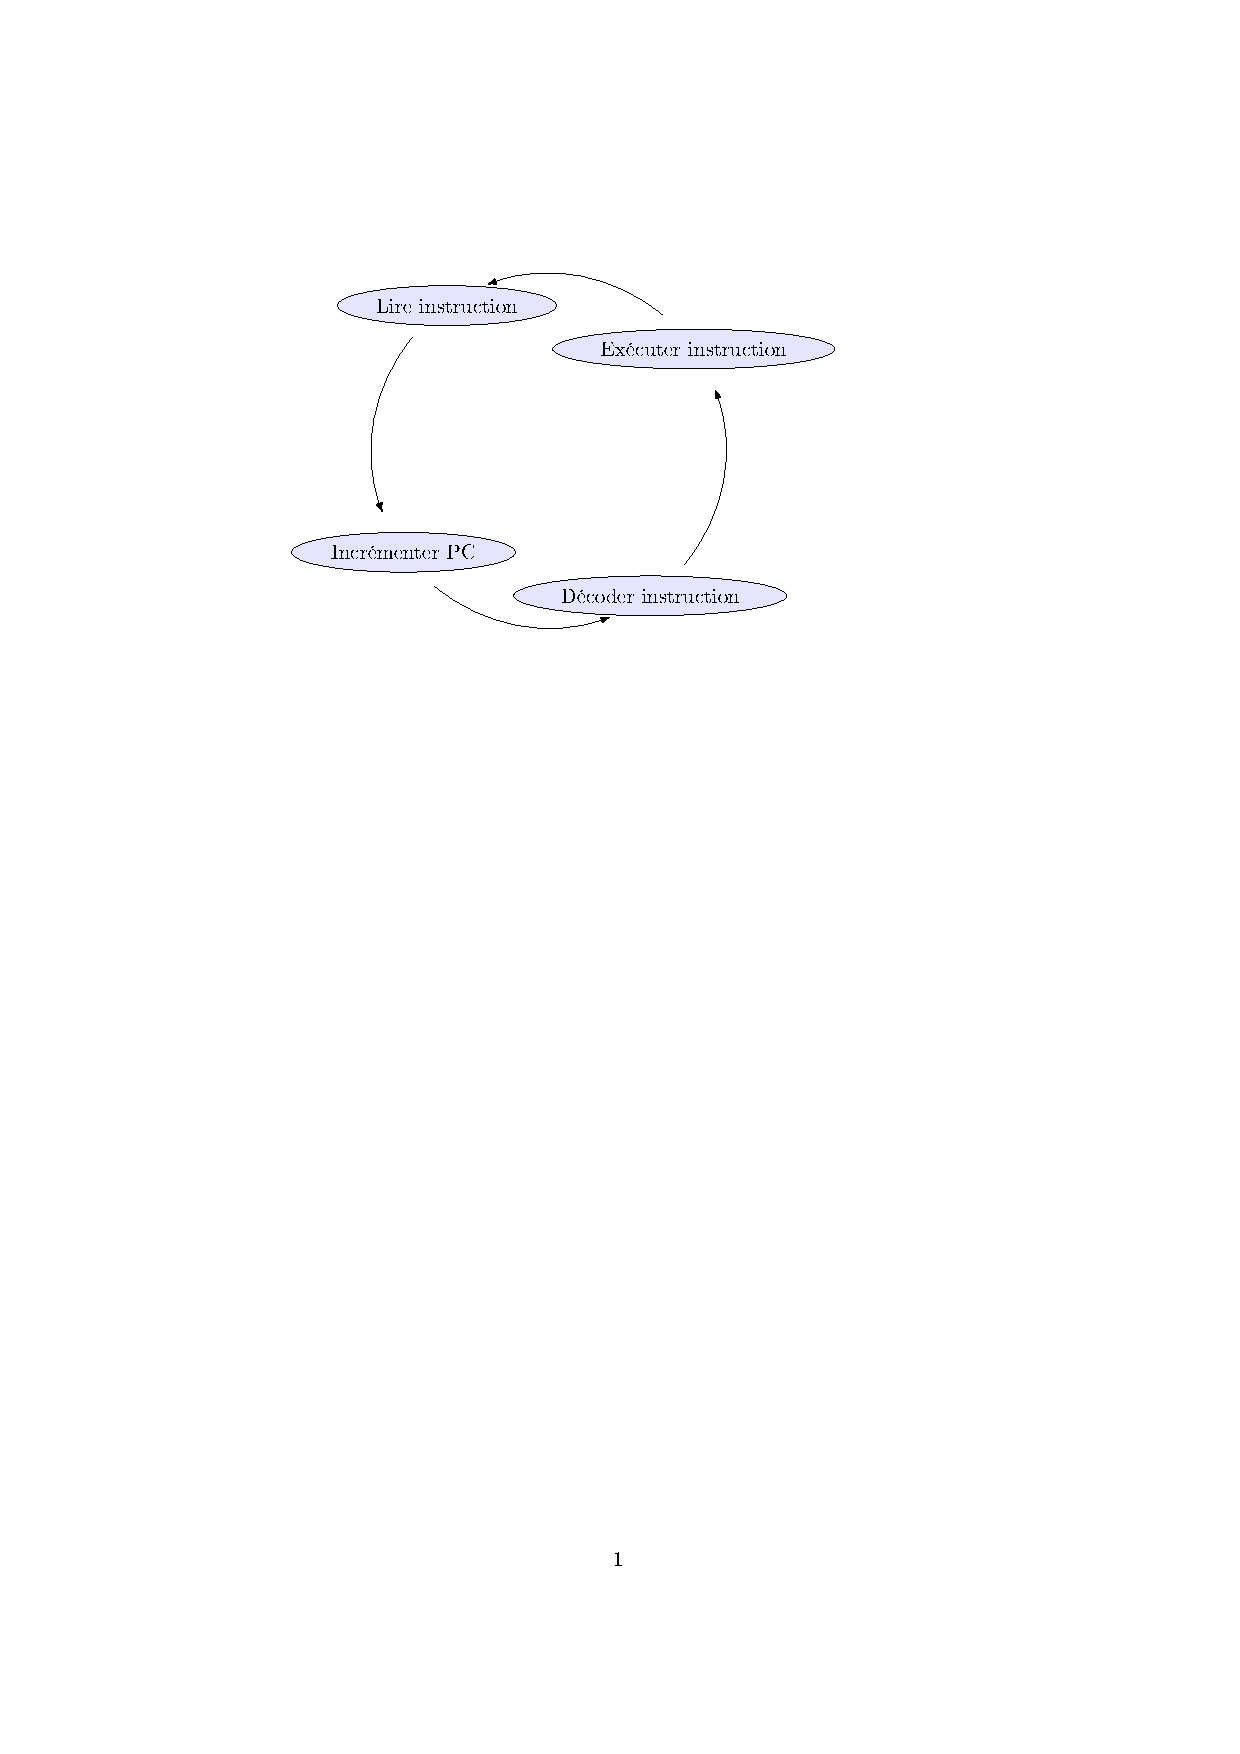
\includegraphics[height=5cm,trim=4.5cm 19cm 6.5cm 4.5cm,clip]{unite-controle.pdf}
  
  {Déroulement schématique des actions effectuées par l'unité de contrôle}

\end{center}

\noindent Avantages de l'architecture de von Neumann:
\begin{itemize}
\item Simplicité conceptuelle
\item Souplesse (peut manipuler tout ce qui est représentable
  numériquement, un programme est une donnée)
\end{itemize}
Inconvénients:
\begin{itemize}
\item Exécution séquentielle
\item Goulet d'étranglement
\item Fragilité (faible robustesse aux erreurs)
\end{itemize}
\subsubsection*{Mise en œuvre}

Problème avec les mémoires vives:
\begin{itemize}
\item Consomment de l'électricité
\item S'effacent quand elles ne sont plus alimentées
\end{itemize}
 
Solutions:
\begin{description}
\item[Mémoire morte (ROM)] Pas besoin d'alimentation mais non
  modifiable. Initialisées à la fabrication. Mémoire d'un PC: un peu
  de ROM, beaucoup de RAM. Contenu de la ROM: firmware (BIOS ou UEFI)
  chargeant le système d'exploitation.
\item[Mémoire de masse] Autrefois lecteur de bande magnétiques,
  aujourd'hui disque dur ou mémoire flash. Grande capacité de stockage
  mais accès plus lent que la RAM (rapport 1000 pour DD/RAM). Stocke
  généralement données utilisateurs + programmes + système d'exploitation.
  plus complexe.
\end{description}

\section*{Objectif du TP : démontage d'un PC et étude de ses composants.}\label{sec.demontage}

Avant tout, notez bien qu'on ne démonte pas les ordinateurs de la
salle de TP mais ceux fournis par l'enseignant dans ce but!

Deuxième chose : on ne touche pas l'intérieur du PC, ou alors le moins
possible et  en ayant pris  soin au préalable  de se décharger  de son
électricité statique en touchant la carcasse du PC.

Chaque  binôme  dispose  d'un PC.  Le  but  du  jeu est  de  l'ouvrir,
d'identifier  les différents  composants (où  est le  disque dur ? la
carte mère ? le processeur ?  la mémoire vive? ), puis de le refermer,
le tout sans casse.

N'oubliez pas de prendre des photos de l'intérieur pour votre
compte-rendu.

\emph{Vous préciserez sur le compte-rendu les différents éléments
  que vous avez identifiés, de préférence à partir de photos.}

\emph{Attention : vous ne démonterez pas ni la carte mère, ni le bloc d'alimentation électrique (vous pourrez ôter ce dernier du l'ordinateur).}  
\end{multicols}